\documentclass[a4paper,12pt]{report}

\usepackage{alltt, fancyvrb, url}
\usepackage{graphicx}
\usepackage[utf8]{inputenc}
\usepackage{float}
\usepackage{hyperref}

% Questo commentalo se vuoi scrivere in inglese.
\usepackage[italian]{babel}

\usepackage[italian]{cleveref}

\title{Relario: Tales of Relano\\Progetto per il corso di\\``Programmazione ad Oggetti''}

\author{Lorenzo Cinelli, Mihai Mazuru, Kimi Osti, Sara Panfini}
\date{\today}


\begin{document}

\maketitle

\tableofcontents

\chapter{Analisi}


\section{Descrizione e requisiti}

Il software realizzato è un videogioco 2D con vista dall’alto. Il suo svolgimento gira attorno a un personaggio principale, controllato dall’utente, che deve attraversare le stanze di un castello per raggiungere lo scontro finale con il Re, di cui deve conquistare il trono.
%
\newline Durante l’esplorazione delle stanze all’utente potranno essere affidate delle quest da completare per poter procedere correttamente.
%
\newline Inoltre, gli verranno presentato delle stanze quasi completamente interattive. In particolare, ci saranno dei personaggi non giocanti (neutri, alleati o nemici) che potranno, al momento dell’interazione, mostrare un messaggio, donare degli oggetti oppure ingaggiare un combattimento. Inoltre, sarà possibile interagire con gran parte degli elementi di arredo presenti in stanza, tra cui elementi come armature o vasi contenenti oggetti collezionabili oppure tappeti o botole che possono celare al loro interno nemici.
%
\newline Il combattimento si svolge per turni. Ad ogni turno, il giocatore può decidere se attaccare o chiedere pietà al nemico, così come può navigare il suo inventario e usare oggetti senza perdere il diritto al turno. Il nemico, in caso venga chiesta pietà, potrebbe concederla oppure rifiutarla e attaccare immediatamente il giocatore. 

\subsubsection{Requisiti funzionali}
\begin{itemize}
	\item I nemici all'interno del gioco saranno di varie tipologie, e dovranno offrire un comportamento variabile all'utente per quanto riguarda le richieste di pietà;
	\item L'arredo delle stanze viene generato casualmente garantendo l'assenza di sovrapposizioni, e le diverse tipologie di elementi di arredo devono offrire diversi scenari di interazione;
	\item Le quest devono essere di diverse tipologie e richiedere diverse azioni da parte del giocatore;
	\item Il combattimento finale deve poter offrire una scelta al giocatore, che sarà in grado di avviare finali diversi.
\end{itemize}

\subsubsection{Requisiti non funzionali}
\begin{itemize}
	\item Per offire un'esperienza gradevole all'utente, si mira a realizzare un software efficiente.
	\item Il software sarà portabile su tutti i maggiori sistemi operativi.
\end{itemize}


\section{Modello del Dominio}

Il dominio applicativo dell’applicazione viene modellato in ogni momento dal concetto di stanza, ovvero il “container” all’interno di cui si svolge la fase centrale del gioco. All’interno della stanza, oltre al personaggio principale, si trovano altre entità, che possono essere personaggi viventi non giocanti (nemici o generici NPC) oppure elementi di arredo. Il giocatore può possedere nel suo inventario diversi oggetti, che vengono anch’essi modellati come entità. In questo scenario, diventa possibile gestire tramite la stanza e le informazioni che ogni entità offre l’intero modello del dominio, estraendo le istanze di interesse per gestire le situazioni contingenti come il combattimento. 
%
\newline Per quanto riguarda l’arredamento, le entità si dividono in tre tipologie fondamentali: arredamento interattivo, che blocca il movimento ma permette interazione, e può rilasciare un oggetto che il giocatore aggiungerà al proprio inventario al momento dell’interazione; arredamento calpestabile, che non ostruisce il movimento e permette interazione, ma può nascondere un nemico con cui viene avviato il combattimento non appena vi si interagisce; arredamento passivo, che ostacola il movimento e non permette alcun tipo di interazione. 
%
\newline Per quanto riguarda i nemici, ad ognuno viene associato un tipo, che ne definisce il livello di difficoltà. Quando viene sconfitto, un nemico rilascia un oggetto di inventario che il giocatore aggiungerà al proprio inventario al momento della vittoria. Ad ogni nemico viene poi associato un comportamento in caso di richieste di pietà, indipendente dal tipo e proprio di ogni singola istanza. In caso il giocatore venga risparmiato dal nemico, non ottiene il suo bottino.
%
\newline Gli NPC modellano tutti i personaggi non ostili all’interno del gioco, con cui sarà possibile interagire in ogni momento. Anche loro possono rilasciare oggetti di inventario al momento dell’interazione, oppure mostrare messaggi, che potranno o meno aiutare il giocatore a completare la quest.
%
\newline Il personaggio principale, che si muove nella mappa e interagisce con il resto delle entità presenti, può portare con sé alcuni oggetti di inventario ottenuti interagendo con le altre entità. Questi oggetti possono essere di vario tipo, e a seconda della tipologia offrire diversi effetti (cura, aumento del danno per le armi e protezione per le armature, oppure nessuno per gli oggetti collezionabili). Le armi e le armature, per essere effettive, devono essere equipaggiate, e hanno una durabilità limitata. Al momento dell’uso dell’oggetto, il suo effetto viene attivato sul giocatore. Un oggetto qualsiasi può anche essere scartato per liberare spazio nell’inventario, che ha capacità limitata.


\begin{figure}[H]
	\centering{}
	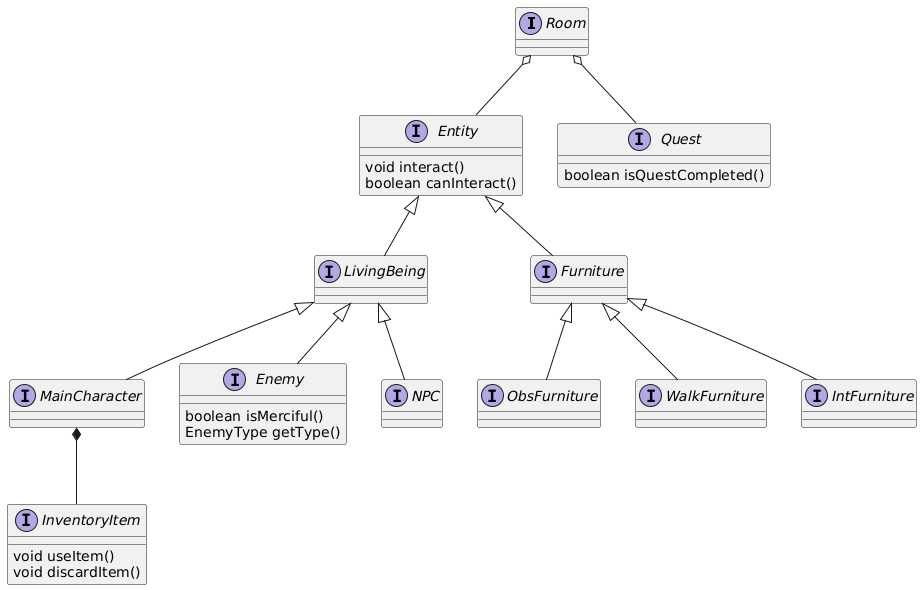
\includegraphics[width=\textwidth]{img/model.png}
	\caption{Schema UML del dominio applicativo}
	\label{img:model}
\end{figure}


\chapter{Design}

\section{Architettura}

Il software si basa sull’architettura MVC nella sua declinazione standard. In particolare, ogni elemento dell’architettura offre un unico entry point verso l’esterno, in modo che gli accessi alle sue funzionalità possano essere uniformi e consistenti, offrendo un ulteriore grado di incapsulamento.
%
\newline Il Model offre come proprio entry point l’interfaccia Room, che fa da scenario base per lo svolgimento della fase di esplorazione del gioco. All’interno della stanza infatti, sono presenti tutte le entità, che vengono modificate ad ogni tick del motore fisico tramite un metodo offerto dalla stessa Room, deputata a controllare anche se le singole entità siano in grado di muoversi al suo interno. 
%
\newline Il Controller, che conserva il riferimento alla stanza in cui attualmente si trova il gioco, gestisce al suo interno le transizioni di stato per le varie fasi del gameplay, interrogando la View per mostrare le interfacce corrette e richiedendo al Model eventuali modifiche. Il Controller è anche responsabile della temporizzazione dell’aggiornamento del motore di gioco, e della traduzione delle entità del Model in elementi rappresentabili correttamente dalla View.
%
\newline La View offre un entry point centrale da cui è possibile richiedere di mostrare le varie interfacce, o l’accesso ai loro riferimenti per chiamare procedure proprie di tali istanze. Nell’architettura realizzata, la View agisce come elemento passivo ricevendo i dati da mostrare dal Controller tramite opportune interrogazioni. La gestione dell’input permette alla View di comunicare particolari eventi al Controller, che li gestirà e ne rifletterà eventualmente gli effetti sul Model.
%
\newline Nella realizzazione dell’architettura MVC, modificare la View non impatta minimamente il Model, dal momento che è solamente il Controller a dialogare con questa componente. Dall’altro lato, il Controller potrebbe essere impattato da una modifica della View radicale (come per esempio trasformare la GUI attiva in un’interfaccia reattiva, oppure la rimozione dei suoni), mentre non sarebbe impattato da modifiche nelle tecniche implementative della GUI - come per esempio una modifica della libreria grafica - a patto che sia in grado di rispettare il contratto stabilito dalle due interfacce (ad esempio accettare gli stessi tipi di chiamate parametrizzate).


\begin{figure}[H]
	\centering{}
	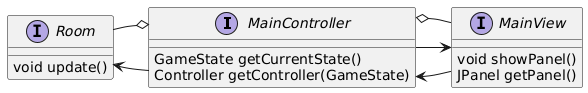
\includegraphics[width=\textwidth]{img/mvc.png}
	\caption{Schema UML degli entry point dei rapporti fra componenti di MVC}
	\label{img:mvc}
\end{figure}

\section{Design dettagliato}



\chapter{Sviluppo}

\section{Testing automatizzato}

Per quanto riguarda il testing automatizzato, si è sfruttata la libreria JUnit e si sono realizzati test su quasi tutte le classi di Model e Controller. Ciò è stato fatto per garantire il corretto funzionamento dell’applicazione, e per avere la certezza che gli eventuali problemi riscontrati durante il gioco non fossero dovuti a mancanze di logica implementativa, quanto a problematiche di visualizzazione. 
%
\newline La View, invece, è stata testata manualmente in fase di sviluppo, e poi in fase di collaudo del software, perché personalmente non siamo riusciti ad approfondire le dinamiche di testing automatizzato che avrebbero permesso di testare automaticamente anche quella parte del software.
%
\newline In linea generale, gli aspetti su cui il testing si è maggiormente soffermato sono stati i seguenti:

\begin{itemize}
	\item Generazione della mappa, movimento e interazioni al suo interno. Particolarmente, si è verificato che il movimento e le interazioni non generassero comportamenti imprevisti e che si riflettessero correttamente sugli aggiornamenti del Model.
	\item Combattimento. In particolare, il testing si concentra sul mantenimento dell’ordine dei turni per evitare comportamenti imprevisti, e sul corretto inserimento in inventario del bottino dei nemici sconfitti.
	\item Protagonista. In particolare, si è testato il sistema di gestione della vita del protagonista, così come del suo inventario. Nei controlli sull’inventario, si è verificato il corretto utilizzo degli oggetti curativi, così come delle armi e armature, per garantire comportamenti consistenti in fase di combattimento.
	\item Input utente. Si sono testati i Controller che svolgono la funzione di Observer, per garantire la corretta gestione degli input.
	\item Creazione delle istanze. Avendo fatto largo uso del Pattern Factory, si è deciso di testare i metodi di generazione degli oggetti per verificare l’effettiva consistenza delle istanze create e garantire prevedibilità in fase di gioco.
\end{itemize}

\section{Note di sviluppo}

\subsection{Kimi Osti}

Di seguito si presentano singoli esempi di uso di costrutti avanzati di Java. Ciò non impedisce che all'interno del codice appaiano più istanze in cui vengono usati.

\subsubsection{Uso di Java Wildcards}
Permalink: \url{https://github.com/KimboCoffee/OOP23-relario/blob/d67fe167022e08cef63d110da0710154eb543292/src/main/java/it/unibo/oop/relario/utils/impl/GameTexturesLocator.java#L42}

\subsubsection{Uso di Lambda Expressions e di Optional}
Permalink: \url{https://github.com/KimboCoffee/OOP23-relario/blob/d67fe167022e08cef63d110da0710154eb543292/src/main/java/it/unibo/oop/relario/model/inventory/InventoryImpl.java#L40}

\subsubsection{Uso di InputStream}
Permalink: \url{https://github.com/KimboCoffee/OOP23-relario/blob/d67fe167022e08cef63d110da0710154eb543292/src/main/java/it/unibo/oop/relario/view/impl/UserGuide.java#L54}

\subsubsection{Gestione esplicita dei Thread}
Permalink: \url{https://github.com/KimboCoffee/OOP23-relario/blame/d67fe167022e08cef63d110da0710154eb543292/src/main/java/it/unibo/oop/relario/controller/impl/GameLoop.java#L32}

\subsubsection{Codice reperito online}
Per la realizzazione della classe BackgroundTile (Permalink:  \url{https://github.com/KimboCoffee/OOP23-relario/blob/d67fe167022e08cef63d110da0710154eb543292/src/main/java/it/unibo/oop/relario/view/impl/BackgroundTile.java}) si è preso spunto da \href{https://coderanch.com/t/336043/java/Images-top}{questa pagina di forum online}.

\chapter{Commenti finali}

\section{Autovalutazione e lavori futuri}

\subsection{Kimi Osti}
Personalmente, questo è stato il primo progetto di gruppo di queste dimensioni a cui mi sono dedicato, e in particolare è stato il primo progetto a cui mi sono dedicato in ambito di videogiochi, tema che mi ha sempre molto affascinato e a cui vorrei dedicare anche la mia carriera futura. In particolare per questo motivo, ho trovato stimolante la fase di sviluppo del software e particolarmente gratificante riuscire a produrre un risultato finale funzionante.
\newline Per quanto riguarda lo sviluppo del software - guardando indietro alle fasi iniziali del progetto - posso dire di ritenermi abbastanza soddisfatto. Durante il corso del progetto ho principalmente appreso alcune delle dinamiche nello sviluppo di software di dimensioni più grandi rispetto ai soliti progetti individuali a cui mi ero dedicato in precedenza, e ho anche capito alcuni concetti che - prima di iniziare a lavorare su questo progetto - non avrei saputo affrontare. Pertanto, posso dire che questo progetto mi è servito individualmente a maturare ulteriormente, e che se dovessi tornare indietro probabilmente lavorerei in modo diverso non tanto per modificare il risultato finale (che si è dimostrato abbastanza vicino a quello che mi ero prefigurato prima di iniziare il lavoro), quanto più in virtù delle dinamiche che ho appreso durante il lavoro e che avrebbero permesso di produrre software in maniera più efficiente.
\newline Per quanto riguarda le dinamiche di gruppo, posso dirmi abbastanza soddisfatto, soprattutto per il fatto che, anche se in alcune fasi vi sono state divergenze di vedute su alcune tematiche, non si sia mai arrivati a situazioni critiche che abbiano pregiudicato lo svolgimento del lavoro. Fin da prima di presentare il progetto, però, sono stato io a presentare l'idea su cui poi si è sviluppato il gioco, e durante il progetto - complice la fiducia che i miei compagni hanno riposto in me - ho assunto il ruolo di "coordinatore" del lavoro. Questo ha però inevitabilmente significato che gran parte delle idee su cui si basa il modello del gioco siano arrivate da me, e che poi io mi sia trovato - soprattutto nelle fasi finali - ad affrontare personalmente le fasi di sviluppo più delicate, come per esempio la soluzione di possibili bug sottolineati dagli strumenti di analisi statica del codice oppure la soluzione del problema di mancato caricamento delle risorse che si è presentata quando abbiamo assemblato il jar per la consegna finale.
\newline Nel complesso però, mi sento di dire che il risultato finale rispecchia abbastanza l'idea che avevo del gioco prima di iniziare lo sviluppo, e che ho trovato stimolante il processo di realizzazione. Per come è strutturato il software ci sarebbe margine per allargarlo e portarlo a qualcosa di più di una demo da qualche minuto, anche se dubito che possa accadere. D'altro canto, personalmente vedo rafforzata la mia passione verso il mondo dello sviluppo di videogiochi, e sono volenteroso di portare avanti questa passione anche con progetti personali che possano permettermi di approfondire ulteriormente parti dello sviluppo che per motivi di suddivisione del lavoro ho toccato meno.

\section{Difficoltà incontrate e commenti per i docenti}

Questa sezione, \textbf{opzionale}, può essere utilizzata per segnalare ai docenti eventuali problemi o difficoltà incontrate nel corso o nello svolgimento del progetto, può essere vista come una seconda possibilità di valutare il corso (dopo quella offerta dalle rilevazioni della didattica) avendo anche conoscenza delle modalità e delle difficoltà collegate all'esame, cosa impossibile da fare usando le valutazioni in aula per ovvie ragioni.
%
È possibile che alcuni dei commenti forniti vengano utilizzati per migliorare il corso in futuro: sebbene non andrà a vostro beneficio, potreste fare un favore ai vostri futuri colleghi.
%
Ovviamente \textit{il contenuto della sezione non impatterà il voto finale}.

\appendix
\chapter{Guida utente}

Capitolo in cui si spiega come utilizzare il software. Nel caso in cui il suo uso sia del tutto
banale, tale capitolo può essere omesso.
%
A tal riguardo, si fa presente agli studenti che i docenti non hanno mai utilizzato il software
prima, per cui aspetti che sembrano del tutto banali a chi ha sviluppato l'applicazione possono non
esserlo per chi la usa per la prima volta.
%
Se, ad esempio, per cominciare una partita con un videogioco è necessario premere la barra
spaziatrice, o il tasto ``P'', è necessario che gli studenti lo segnalino.

\subsection*{Elementi positivi}

\begin{itemize}
 \item Si istruisce in modo semplice l'utente sull'uso dell'applicazione, eventualmente facendo uso di schermate e descrizioni.
\end{itemize}

\subsection*{Elementi negativi}
\begin{itemize}
 \item Si descrivono in modo eccessivamente minuzioso tutte le caratteristiche, anche minori, del software in oggetto.
 \item Manca una descrizione che consenta ad un utente qualunque di utilizzare almeno le funzionalità primarie dell'applicativo.
\end{itemize}

\chapter{Esercitazioni di laboratorio}

In questo capitolo ciascuno studente elenca gli esercizi di laboratorio che ha svolto
(se ne ha svolti),
elencando i permalink dei post sul forum dove è avvenuta la consegna.
%
Questa sezione potrebbe essere processata da strumenti automatici,
per cui link a oggetti diversi dal permalink della consegna,
errori nell'email o nel nome del laboratorio possono portare ad ignorare alcune consegne,
si raccomanda la massima precisione.

\section*{Esempio}

\subsection{paolino.paperino@studio.unibo.it}

\begin{itemize}
 \item Laboratorio 04: \url{https://virtuale.unibo.it/mod/forum/discuss.php?d=12345#p123456}
 \item Laboratorio 06: \url{https://virtuale.unibo.it/mod/forum/discuss.php?d=22222#p222222}
 \item Laboratorio 09: \url{https://virtuale.unibo.it/mod/forum/discuss.php?d=99999#p999999}
\end{itemize}

\subsection{paperon.depaperoni@studio.unibo.it}

\begin{itemize}
 \item Laboratorio 04: \url{https://virtuale.unibo.it/mod/forum/discuss.php?d=12345#p123456}
 \item Laboratorio 05: \url{https://virtuale.unibo.it/mod/forum/discuss.php?d=22222#p222222}
 \item Laboratorio 06: \url{https://virtuale.unibo.it/mod/forum/discuss.php?d=99999#p999999}
 \item Laboratorio 07: \url{https://virtuale.unibo.it/mod/forum/discuss.php?d=22222#p222222}
 \item Laboratorio 08: \url{https://virtuale.unibo.it/mod/forum/discuss.php?d=99999#p999999}
 \item Laboratorio 09: \url{https://virtuale.unibo.it/mod/forum/discuss.php?d=22222#p222222}
 \item Laboratorio 10: \url{https://virtuale.unibo.it/mod/forum/discuss.php?d=99999#p999999}
 \item Laboratorio 11: \url{https://virtuale.unibo.it/mod/forum/discuss.php?d=22222#p222222}
\end{itemize}


\bibliographystyle{alpha}
\bibliography{13-template}

\end{document}
